%!TEX root = ../main.tex
%
% モンテカルロ法によるシミュレーション
% レポート用紙
%

\stepcounter{section}
\section*{モンテカルロ法によるシミュレーション}

\begin{center}
\begin{tabular}{|c|c|c|c|}
\hline
\parbox[c][1.2cm][c]{0cm}{}学籍番号 & \hspace{3cm} & 名前 & \hspace{6cm} \\
\hline
\parbox[c][1.2cm][c]{0cm}{}実験日時 & \multicolumn{3}{|l|}{   年  月  日  曜日  時限}\\
\hline
\parbox[c][2.0cm][c]{0cm}{}共同実験者 & \multicolumn{3}{|l|}{}\\
\hline
\end{tabular}
\end{center}

\subsection*{実験の目的}

\vspace{2cm}


\subsection*{測定値および計算}

\subjikken{}

\subsubsection*{測定値}

\hspace*{-\parindent}
{\small 乱数サイの色と組:
$x$座標用(10の位 色、1の位 色)、$y$座標用(10の位 色、1の位 色)}

\bigskip

\hspace*{-\parindent}
\begin{tabular}{|c|c|c|c|c|c|c|c|c|c|c|c|c|c|c|c|c|c|c|c|}
\hline
\scriptsize 回 & \scriptsize 座標 & \scriptsize 回 & \scriptsize 座標 & \scriptsize 回 & \scriptsize 座標 & \scriptsize 回 & \scriptsize 座標 & \scriptsize 回 & \scriptsize 座標 & \scriptsize 回 & \scriptsize 座標 & \scriptsize 回 & \scriptsize 座標 & \scriptsize 回 & \scriptsize 座標 & \scriptsize 回 & \scriptsize 座標 & \scriptsize 回 & \scriptsize 座標 \\
\hline\hline
\scriptsize 1 & & \scriptsize 11 && \scriptsize 21 && \scriptsize 31 && \scriptsize 41 && \scriptsize 51 && \scriptsize 61 && \scriptsize 71 && \scriptsize 81 && \scriptsize 91 & \\
\hline
\scriptsize 2 & & \scriptsize 12 && \scriptsize 22 && \scriptsize 32 && \scriptsize 42 && \scriptsize 52 && \scriptsize 62 && \scriptsize 72 && \scriptsize 82 && \scriptsize 92 & \\
\hline
\scriptsize 3 & & \scriptsize 13 && \scriptsize 23 && \scriptsize 33 && \scriptsize 43 && \scriptsize 53 && \scriptsize 63 && \scriptsize 73 && \scriptsize 83 && \scriptsize 93 & \\
\hline
\scriptsize 4 & & \scriptsize 14 && \scriptsize 24 && \scriptsize 34 && \scriptsize 44 && \scriptsize 54 && \scriptsize 64 && \scriptsize 74 && \scriptsize 84 && \scriptsize 94 & \\
\hline
\scriptsize 5 & & \scriptsize 15 && \scriptsize 25 && \scriptsize 35 && \scriptsize 45 && \scriptsize 55 && \scriptsize 65 && \scriptsize 75 && \scriptsize 85 && \scriptsize 95 & \\
\hline
\scriptsize 6 & & \scriptsize 16 && \scriptsize 26 && \scriptsize 36 && \scriptsize 46 && \scriptsize 56 && \scriptsize 66 && \scriptsize 76 && \scriptsize 86 && \scriptsize 96 & \\
\hline
\scriptsize 7 & & \scriptsize 17 && \scriptsize 27 && \scriptsize 37 && \scriptsize 47 && \scriptsize 57 && \scriptsize 67 && \scriptsize 77 && \scriptsize 87 && \scriptsize 97 & \\
\hline
\scriptsize 8 & & \scriptsize 18 && \scriptsize 28 && \scriptsize 38 && \scriptsize 48 && \scriptsize 58 && \scriptsize 68 && \scriptsize 78 && \scriptsize 88 && \scriptsize 98 & \\
\hline
\scriptsize 9& & \scriptsize 19 && \scriptsize 29 && \scriptsize 39 && \scriptsize 49 && \scriptsize 59 && \scriptsize 69 && \scriptsize 79 && \scriptsize 89 && \scriptsize 99 & \\
\hline
\scriptsize 10 & & \scriptsize 20 && \scriptsize 30 && \scriptsize 40 && \scriptsize 50 && \scriptsize 60 && \scriptsize 70 && \scriptsize 80 && \scriptsize 90 && \scriptsize 100 & \\
\hline
\end{tabular}

\newpage

\subsubsection*{結果のプロット}

\hspace*{-\parindent}
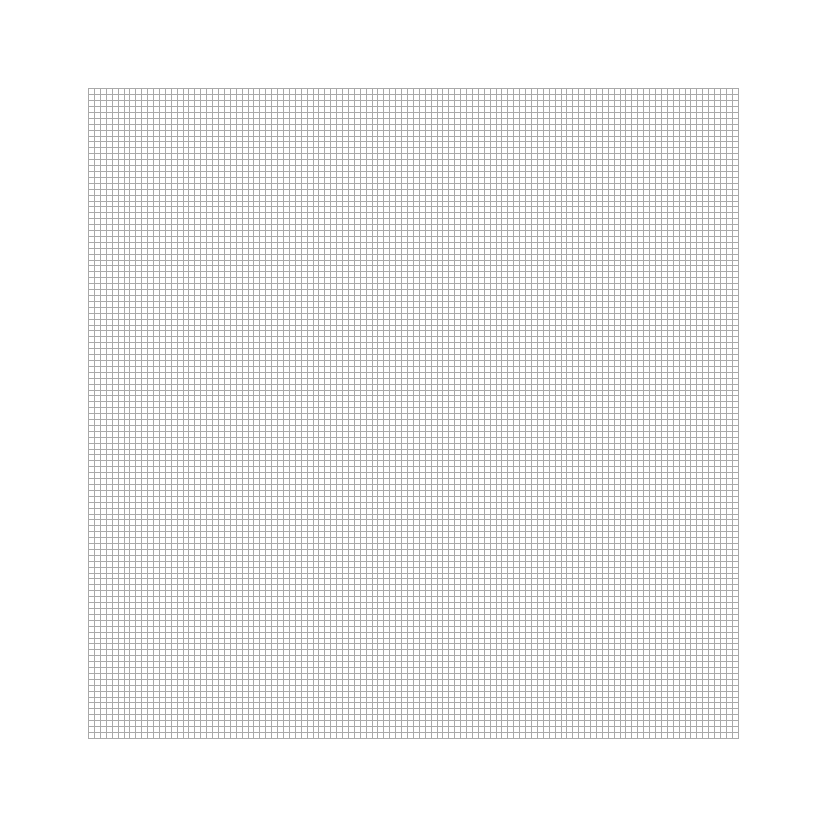
\includegraphics[bb=33 32 365 362]{08_MonteCarlo/graph.pdf}

\subsubsection*{集計}

\hspace*{-\parindent}
\begin{tabular}{|c|c|c|c|c|}
\hline
& 1〜25 & 26〜50 & 51〜75 & 76〜100\\
\hline
内部の点の数 $p$ & & & & \\
\hline
外部の点の数 $q$ & & & & \\
\hline
 & \hspace*{2.5cm} & \hspace*{2.5cm} & \hspace*{2.5cm} & \hspace*{2.5cm}\\
\cline{2-5}
$\frac{4p}{p+q}=\pi$ & \multicolumn{2}{|c|}{} &  \multicolumn{2}{|c|}{} \\
\cline{2-5}
 & \multicolumn{4}{|c|}{} \\
\hline
\end{tabular}

\newpage

\subjikken{}

\hspace*{-\parindent}
\begin{tabular}{|c|c|c|c|}
\hline
& サイコロを振る回数 & 計算の繰り返し回数 & 得られた円周率の値 \\
\hline\hline
1&&&\\
\hline
2&&&\\
\hline
3&&&\\
\hline
4&&&\\
\hline
5&&&\\
\hline
\end{tabular}

%\newpage

\subsection*{考察}

